\documentclass[aps,prd,twocolumn,10pt,superscriptaddress,nofootinbib,longbibliography,floatfix]{revtex4-2}

\usepackage{amsmath,amssymb,amsfonts}
\usepackage{bm}
\usepackage{graphicx}
\usepackage{booktabs}
\usepackage{xcolor}
\usepackage{hyperref}
\graphicspath{{figures/}}
\hypersetup{colorlinks=true,linkcolor=blue,citecolor=blue,urlcolor=blue}

\newcommand{\dd}{\mathrm{d}}
\newcommand{\Ham}{\mathcal{H}}
\newcommand{\Mom}{\mathcal{M}}
\newcommand{\TT}{\Lambda}
\newcommand{\Hc}{\mathcal{H}_c}

\begin{document}

\title{Gravitational waves from structure formation in an early matter era:\\ Scope, set-up, and first tests (working note v0)}

\author{Track B of the numerical-relativity particle-in-cell cosmology program}

\date{Working note v0, state of 15 November 2026}

\begin{abstract}
An early era dominated by pressureless matter lets small density fluctuations grow into collapsed structure long before the radiation era begins, and the collapse, virialization and merging of that structure radiate gravitational waves. Every estimate of this signal so far uses Newtonian gravity and the quadrupole formula, although the matter reaches a sizable fraction of the speed of light near the emission peak. This working note scopes a calculation of the signal in full general relativity, with collisionless particles coupled to a numerical-relativity evolution of the spacetime in a periodic expanding box. An exactly plane-symmetric pancake radiates nothing, so the first source is a family of two crossed sine waves whose single-wave member is a built-in null and whose strain before shell crossing has a closed form at second order. The tests done so far show that the box propagates an exact gravitational wave with the errors its finite differences predict, that two independent diagnostics recover the wave from the code's output, and that a plane-wave pancake evolves through shell crossing in full general relativity with every particle kept. Its departure from the Newtonian solution is converged and grows with the square of the ratio of the Hubble radius to the wavelength, and its constraint violation before crossing is the sampling error of a stretched particle lattice, which a finer lattice removes. A semi-analytic Newtonian baseline reproduces the power law of the literature. The note closes with the scan that comes next and the questions it leaves open.
\end{abstract}

\maketitle

\section{Introduction}\label{sec:intro}

If the early universe passed through an era dominated by pressureless matter, for example a heavy field oscillating before it decays, density fluctuations grew linearly with the scale factor instead of logarithmically, and fluctuations of small primordial amplitude collapsed into halos within the era. The formation, virialization and merging of these halos radiate gravitational waves, a stochastic background that could be the only observable trace of such an era. Two box calculations computed this background from Newtonian $N$-body simulations \cite{Eggemeier:2022gw,Fernandez:2023gw}, the second coupled to a lattice for the radiation, and its authors note that a fully relativistic treatment of gravity is needed to resolve the spectrum at higher frequencies. Two further calculations followed single collapsing patches, a Zel'dovich ellipsoid \cite{Dalianis:2024gw} and an $N$-body ellipsoid \cite{Escriva:2026gw}, with the flat-space quadrupole formula. The representative case of Ref.~\cite{Escriva:2026gw} reaches mean peculiar speeds of a large fraction of the speed of light at the emission peak, where its authors expect relativistic corrections. The question of this track is therefore twofold: how much gravitational radiation the structure of an early matter era produces, and in which range the Newtonian estimates can be trusted.

Full numerical relativity evolves the metric itself, so the radiative degrees of freedom are part of the solution and no quadrupole formula is needed. The numerical-relativity particle-in-cell method of Wu and Most \cite{Wu:2026nrpic} couples macroparticles on geodesics to the Z4c evolution of the spacetime; this program applies a version of that method, extended to periodic expanding domains, in the code AthenaK \cite{Stone:2024athenak}. Particles are essential here: a pressureless fluid stops at the first shell crossing, while the emission peaks after it. The work is carried out by large-language-model agents under human direction.

This note records the scoping stage. Section~\ref{sec:problem} asks what radiates, fixes the first source and gives its second-order strain. Section~\ref{sec:setup} describes the calculation and its numerical methods. Section~\ref{sec:tests} reports the tests done so far:
(i) the periodic box propagates an exact linear wave with the errors its stencils predict;
(ii) the flat transverse-traceless projection and the Weyl scalar recover that wave from the code's output;
(iii) a plane-wave pancake evolves through shell crossing in full relativity, with a converged departure from Newtonian gravity that grows with the square of the ratio of the Hubble radius to the wavelength;
(iv) the homogeneous background follows the exact solution;
(v) a semi-analytic Newtonian baseline reproduces the power law of the literature.
Section~\ref{sec:plan} gives the plan and what is open. Table~\ref{tab:parameters} holds the parameters of the scenarios, and Table~\ref{tab:ledger} every number behind the note with the registered run that produced it.

\section{What radiates}\label{sec:problem}

\subsection{The plane-symmetric null}\label{sec:null}

The minimum calculation one would write down first is a plane-symmetric pancake: one sine wave of the density in a periodic box, collapsing along one axis into a sheet. It radiates nothing. Data that depend on $x$ alone are invariant under translations and rotations in the $y$--$z$ plane, the Euclidean group $E(2)$. Every symmetric tensor with this symmetry has the form $\mathrm{diag}(A,B,B)$ plus terms along $x$, and the transverse-traceless (TT) projector along the $x$ axis annihilates all of them, so the TT part vanishes at every nonzero wave number. On the torus one global mode survives: the traceless, divergence-free tensor $\mathrm{diag}(1,-\tfrac12,-\tfrac12)$ divided by the cube of the transverse scale factor, an anisotropic mean expansion of the whole box, which carries no radiation. Both statements were checked symbolically and rederived independently.

The same symmetry restricts the relativistic pancake itself. With a transverse metric that depends on time alone, the Einstein equations admit a longitudinal metric of the Zel'dovich form, the transverse one times one plus a growth factor times a profile, only when the growth factor is constant, a relabelling of $x$, or decays as $1/t$. The naive relativistic form of the pancake is thus the decaying mode, and the reference solution of the relativistic pancake has to come from the planar members of the Szekeres class of dust solutions \cite{Bolejko:2018silent}, which we have yet to derive.

\subsection{The first source: crossed waves}\label{sec:source}

The source is therefore a family. Take the potential of two crossed sine waves of unequal amplitude in a box of side $L$,
\begin{equation}\label{eq:potential}
\Phi = \phi_x\sin kx + \phi_y\sin ky,\qquad \phi_i = -\frac32\left(\frac{H}{k}\right)^2\delta\,r_i,
\end{equation}
with $k=2\pi/L$, $H$ the Hubble rate of the initial slice, $\delta$ the linear density contrast there, and amplitude ratios $r=(1,\epsilon,0)$. The member $\epsilon=0$ is the plane-symmetric pancake, the null of the family; for $\epsilon>0$ the products of the two waves source the modes $\mathbf K=(k,\pm k,0)$, which are TT. The weak-field equation for the tensor part of the metric, $\dd s^2=a^2[-(1+2\Phi)\dd\tau^2+(1-2\Phi)\delta_{ij}\dd x^i\dd x^j+h_{ij}\dd x^i\dd x^j]$, is \cite{Adamek:2016gevolution}
\begin{equation}\label{eq:tensor}
\begin{split}
\tfrac12 h''_{ij} + \Hc h'_{ij} - \tfrac12\nabla^2 h_{ij} = \TT_{ij}{}^{kl}\big[&8\pi G a^2\Pi_{kl} - 2\partial_k\Phi\,\partial_l\Phi\\
&- 4\Phi\,\partial_k\partial_l\Phi\big],
\end{split}
\end{equation}
where $\tau$ is conformal time, $\Hc$ the conformal Hubble rate, $\Pi_{kl}$ the anisotropic stress and $\TT$ the TT projector. In the matter era the potential is constant, the velocity is $-(2/3\Hc)\nabla\Phi$, and the projection of $\Phi\,\partial_k\partial_l\Phi$ equals minus that of $\partial_k\Phi\,\partial_l\Phi$, so the source reduces to $\tfrac{10}{3}\TT[\partial\Phi\,\partial\Phi]$. Its quasi-static solution at $\mathbf K=(k,k,0)$ is the crossed-wave strain
\begin{equation}\label{eq:strain}
h_+ = -\frac56\,\phi_x\phi_y\cos(\mathbf K\cdot\mathbf x),
\end{equation}
in the polarization basis $e_+ = uu - zz$ with $u=(1,-1,0)/\sqrt2$; the mode $(k,-k,0)$ carries the opposite sign in its own basis. The strain is linear in $\epsilon$ and of second order in $\delta$. Projecting the source of the weak-field equation on a grid reproduces the coefficient to rounding error over three decades of $\epsilon$, and gives the same amplitude for two and for three equal waves [Fig.~\ref{fig:source}(a)]. The derivation was redone independently by a second agent in real space.

\begin{figure}[t]
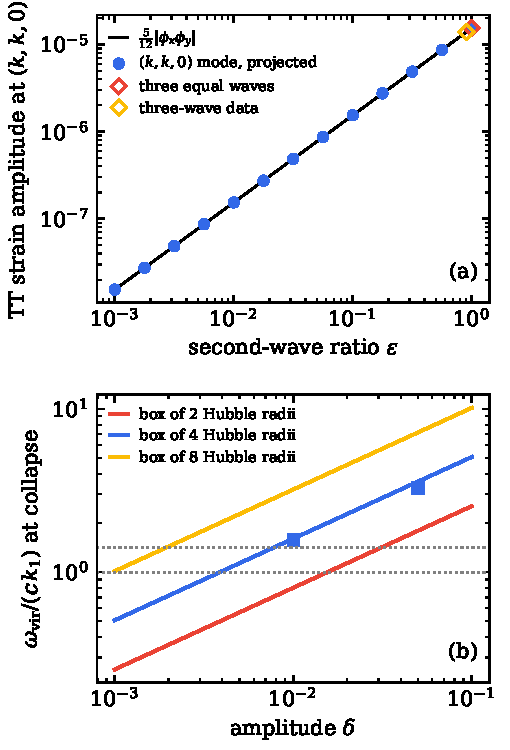
\includegraphics[width=\columnwidth]{fig_source.pdf}
\caption{The first source. (a) TT strain of the $(k,k,0)$ mode against the second-wave ratio (circles) and the closed form (line); diamonds: three equal waves, three-wave data. (b) Virial frequency at collapse over the lowest box wave number for three box sizes; squares: earlier relativistic runs; dotted: $k_1$, $\sqrt2\,k_1$.}
\label{fig:source}
\end{figure}

The initial data of the code are conformally flat, so the TT part starts at zero and approaches the crossed-wave strain through an oscillation, the junk radiation of the data. Writing $h_+(\tau)=h_s\,g(\tau)$ with $h_s$ the static value above, the junk equation
\begin{equation}\label{eq:junk}
g'' + 2\Hc g' + |\mathbf K|^2 (g-1) = 0,\qquad g(0)=g'(0)=0,
\end{equation}
gives an oscillation about one whose envelope falls as $1/a$, the decay of a free wave in the matter era. Both the static strain and the decaying oscillation are predictions for the code before shell crossing.

\subsection{The radiation band and the relativistic depth}\label{sec:band}

A halo radiates near its virial frequency at collapse. For a box of side $L$ the lowest radiating modes are $k_1=2\pi/L$ and $\sqrt2\,k_1$, so the box size decides whether the box modes sample the radiation band or only the near field of the collapse [Fig.~\ref{fig:source}(b)]. In a box of four initial Hubble radii the virial frequency at collapse crosses the two lowest modes within the planned amplitudes; in a box of two it stays below them at small amplitude. The box of four initial Hubble radii is our choice for the first source, with two and eight as the size leg.

The size of the relativistic corrections follows from the depth of the potential,
\begin{equation}\label{eq:depth}
\psi_N = \frac32\left(\frac{H}{k}\right)^2\delta,
\end{equation}
which grows with the square of the box size in Hubble radii. Before shell crossing, Newtonian $N$-body evolution with Zel'dovich data already contains the first-order relativistic effects in a suitable gauge \cite{Fidler:2015za}; the relativistic content of the signal enters through $\psi_N$, through the gauge of the projection, and after shell crossing through the strong compression of the multi-stream region.

\section{The calculation}\label{sec:setup}

\subsection{The expanding periodic box}\label{sec:box}

The universe is a periodic box filled with collisionless particles that start on a lattice displaced by the Zel'dovich growing mode of the potential above. The constraints are solved on the torus spectrally for conformally flat data, following the construction of East, Wojtak and Pretorius \cite{East:2019ev}, which this program's cosmology extension reproduced. The slicing is the conformal-time slicing
\begin{equation}\label{eq:slicing}
\partial_t\alpha = -\tfrac13\alpha^2 K,
\end{equation}
with lapse $\alpha$ and the trace $K$ of the extrinsic curvature; for the homogeneous matter era it keeps $\alpha=a$, so the coordinate time is conformal time. The shift is zero. This is the slicing of the earlier relativistic structure-formation runs of this program; harmonic slicing and the $1+\log$ condition are the gauge leg of the convergence tests. Figure~\ref{fig:architecture} shows the parts of the calculation, which of them exist and which are new.

\begin{figure*}[t]
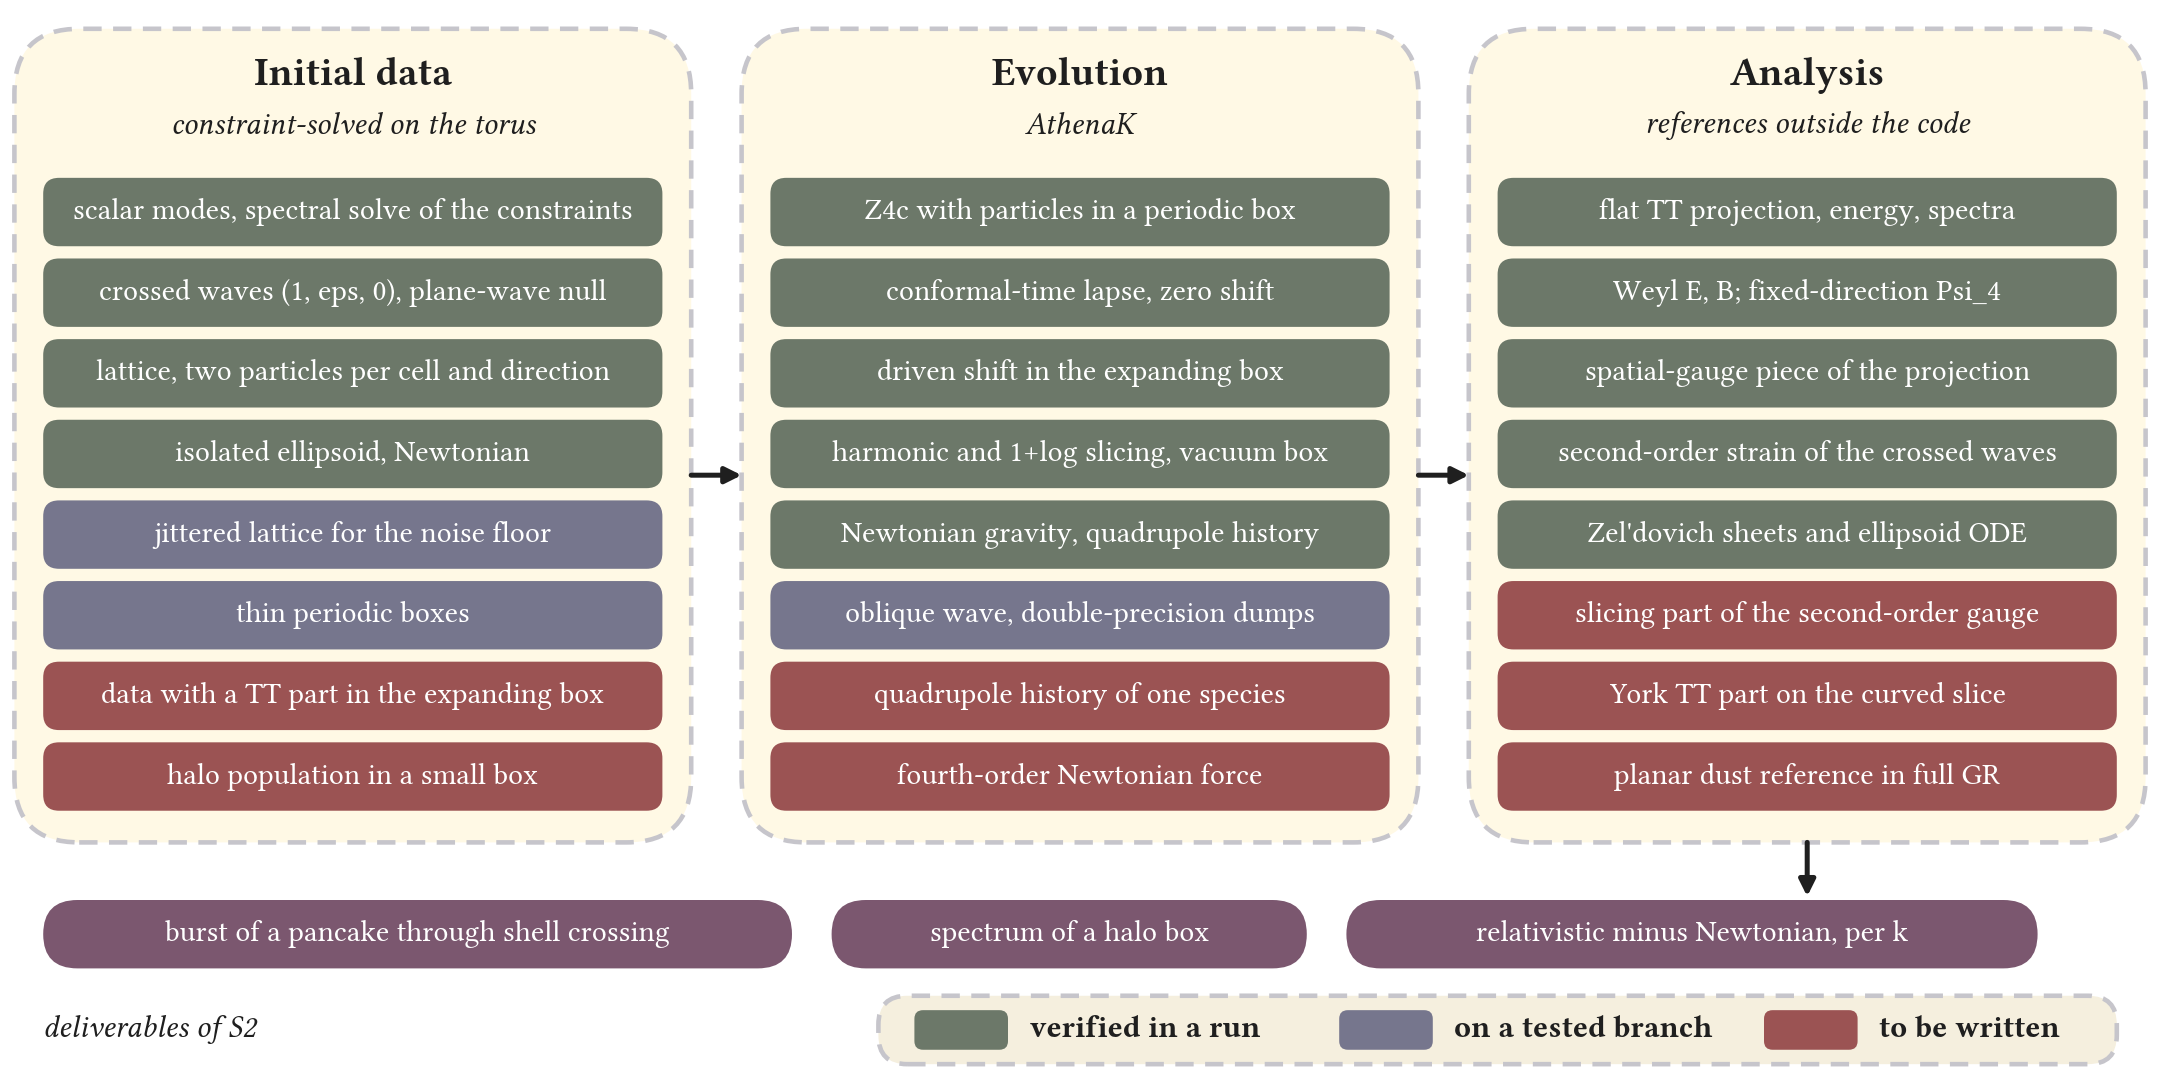
\includegraphics[width=\textwidth]{schem_architecture.png}
\caption{Architecture of the calculation. Columns: initial data, evolution in the code, and analysis with the reference solutions outside the code. Green: exists in this program; slate: exists for another setting and is carried over; red: to be written. Bottom: the deliverables of the problem.}
\label{fig:architecture}
\end{figure*}

\subsection{Gravitational-wave diagnostics}\label{sec:diag}

Two diagnostics measure the radiation. The first is the flat TT projection of the conformal metric perturbation and of the extrinsic curvature in Fourier space, $\TT_{ij,kl}=P_{ik}P_{jl}-\tfrac12P_{ij}P_{kl}$ with $P_{ij}=\delta_{ij}-\hat k_i\hat k_j$. It gives the strain $h^{\rm TT}_{ij}$, its two polarizations and helicities, the spectrum per wave number, and the energy density
\begin{equation}\label{eq:rhoK}
\rho_K = \frac{M_{\rm pl}^2}{2}K^{\rm TT}_{ij}K_{\rm TT}^{ij} = \frac{\langle h'^{\rm TT}_{ij}h'^{ij}_{\rm TT}\rangle}{64\pi G}
\end{equation}
of Ota, Macpherson and Coulton \cite{Ota:2021tt}, where the second form holds for $K_{ij}=-\tfrac12 h'_{ij}$; it is half of the Isaacson energy, the kinetic half. The second diagnostic is the Weyl tensor: its electric and magnetic parts on the slice and the scalar $\Psi_4$ on a null tetrad fixed along the wave direction, which equals $\ddot h_+ - i\,\ddot h_\times$ for a plane wave.

The flat projection is exact at first order. At second order the TT part depends on the slicing and on the spatial coordinates \cite{Hwang:2017gauge}, and the York decomposition on the curved slice, which removes the spatial part of this dependence, is still to be implemented. The magnetic Weyl part vanishes at first order for scalar perturbations and is the gauge-robust check of a second-order signal.

\subsection{Numerical methods}\label{sec:methods}

The spacetime is evolved with the Z4c formulation of AthenaK \cite{Stone:2024athenak} with finite differences of high order, Kreiss--Oliger dissipation, fourth-order Runge--Kutta time integration and constraint damping. The particles follow geodesics; their energy-momentum is deposited with a cubic cloud and a compensation of its smoothing, and the metric is interpolated to them with cubic splines \cite{Wu:2026nrpic}. The step is limited by the expansion as well as by the light crossing of a cell.

Three Newtonian references come with the same initial data. The plane wave has an exact Zel'dovich solution up to shell crossing, written for the discrete sheets of the particle lattice. A particle-mesh code evolves the same particles in Newtonian gravity through shell crossing. For isolated patches, the Zel'dovich ellipsoid and the homogeneous-ellipsoid equations give the quadrupole radiation of Refs.~\cite{Dalianis:2024gw,Escriva:2026gw}. The code now also has a Newtonian mode for the same particles, with the quadrupole history written during the run; its runs are the next baseline (Sec.~\ref{sec:plan}).

\section{Tests so far}\label{sec:tests}

\subsection{Linear waves in the periodic box}\label{sec:linear}

A TT wave of amplitude $10^{-6}$ travelling along $x$ in a vacuum box of one wavelength was evolved for ten crossings at four resolutions and with two sets of numerics, those of the cosmology runs and those of the upstream test input [Fig.~\ref{fig:waves}(a)]. The amplitude error falls at the order of the dissipation term, the phase error at the order of the derivative stencils and the time integrator, and both follow the prediction from the Fourier symbol of the scheme, written before the runs. The largest departure from that prediction is in the phase error at the finest resolution before the floor; at the finest resolution the error stops falling because the perturbation $1+h$ is rounded, and the departure there scales as the inverse amplitude. Fields that vanish at first order grow as the square of the amplitude times the square of the time, the closed-box backreaction of the wave on the mean expansion, with the lapse change of the slicing in use; a second agent derived both coefficients.

The upstream generator of linear waves writes data that are TT only for wave vectors along an axis: for an oblique wave vector two signs of its polarization tensor are reversed, and the data violate both constraints at first order. Flipping the two signs makes the tensor transverse for every direction. The oblique test therefore waits for that fix in the code. A gauge wave in harmonic slicing converges at the order of the scheme. A record of the lapse and shift options in a vacuum box shows that the conformal-time slicing, like the volume slicing, forms a gauge shock within two crossings when the extrinsic curvature varies across the box by a sizable fraction of the wave number, while harmonic slicing stays smooth; this bounds the regime in which the production slicing can be trusted after collapse.

\begin{figure}[t]
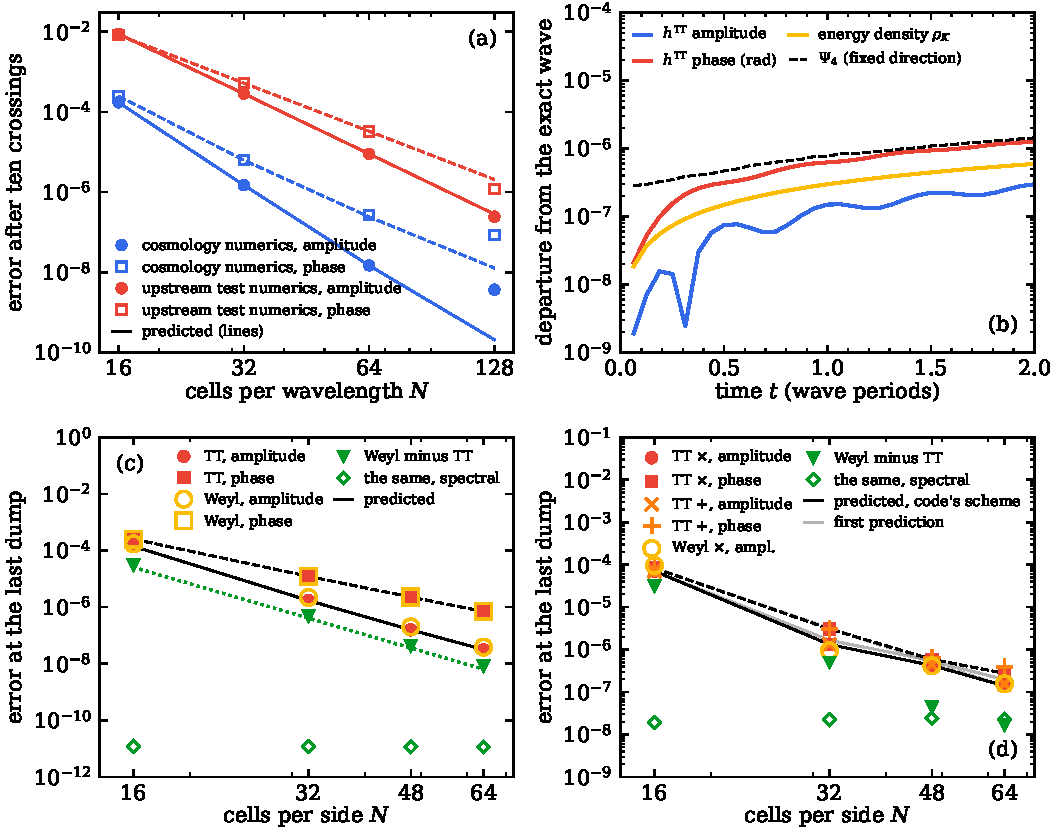
\includegraphics[width=\columnwidth]{fig_waves.pdf}
\caption{A linear wave in the periodic vacuum box. (a) Amplitude (filled) and phase (open) errors after ten crossings, two sets of numerics; lines: Fourier-symbol prediction. (b) Departure of the projected strain, its energy density and the fixed-direction $\Psi_4$ from the exact wave, one run with 32 cells.}
\label{fig:waves}
\end{figure}

\subsection{The diagnostics on code output}\label{sec:diagtests}

On analytic fields, a superposition of random TT waves, the projection returns the energy of every spectral shell to rounding error, separates the helicities, and assigns nothing to a pure-gauge or scalar field at first order. On the dumps of an AthenaK wave over two periods [Fig.~\ref{fig:waves}(b)], the projected amplitude and phase depart from the exact wave by the discretization error of the evolution itself, consistent with the convergence test at the same resolution, and the energy density follows. The fixed-direction $\Psi_4$ computed from the same dumps equals the second time derivative of the exact strain to the same level. The code's own Weyl output lags the dump by a fixed number of steps and uses a tetrad built from the radial direction, so its value depends on the position for a plane wave; the fixed-direction scalar replaces it for this problem.

Applied to the dumps of an earlier relativistic run of three crossed waves, the projection finds a TT strain that freezes at the expected size before collapse and rises late, after the scale factor has grown by several hundred. The late rise coincides with the square of the non-TT part of the metric reaching the TT level, the size of the second-order gauge piece of the flat projection in zero shift; until the gauge test of Sec.~\ref{sec:plan} has run, the rise is a candidate gauge effect.

\subsection{The pancake through shell crossing}\label{sec:pancake}

The plane-wave pancake, the null member of the family, was evolved in full relativity with amplitude $\delta=0.05$ in boxes of one and four initial Hubble radii, at three resolutions and with one and with two particles per cell and direction, to twice the scale factor of the first crossing. Every run reached the end with every particle kept, and the plane symmetry held to rounding error in positions and transverse velocities through the multi-stream region. The first crossing comes slightly later than for the exact Zel'dovich sheets, more so at coarse resolution, where the cloud smooths a sheet thinner than a cell, and approaches the exact value with resolution; the Newtonian particle-mesh run shows the same.

The relativistic coordinate positions depart from the Newtonian ones by a smooth pattern of the first and second harmonics of the box, with no structure at the cell scale. This departure is the same at 32, 64 and 96 cells and with two particles per cell and direction, so it is a property of the solution in these coordinates. Divided by 16, the ratio of $(H/k)^2$ between the two boxes, the departure in the large box falls on top of the small-box curves after the first few units of time [Fig.~\ref{fig:pancake}(a)]: the relativistic correction to the coordinate trajectories scales as $(H/k)^2\delta$, as the depth of the potential predicts. In the proper time of the crossing sheets the large box also crosses later. The early mismatch of the large box is an oscillation with a period close to one light crossing of the box, a transient of the initial data that we have yet to identify.

\begin{figure}[t]
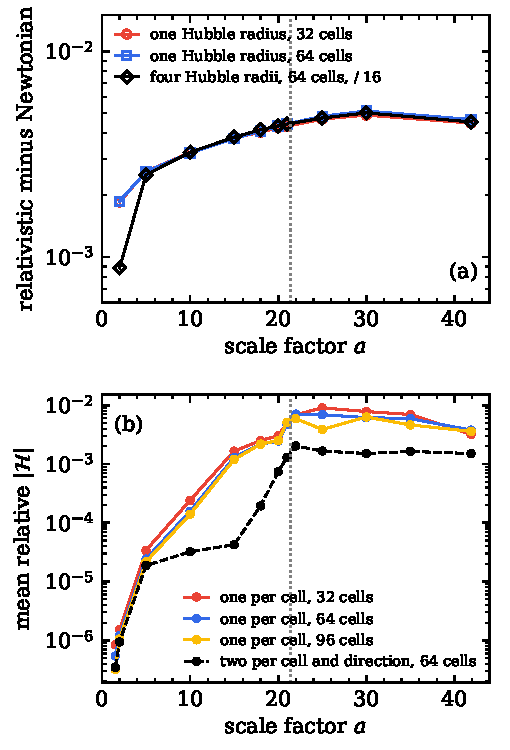
\includegraphics[width=\columnwidth]{fig_pancake.pdf}
\caption{The plane-wave pancake in full relativity. (a) Largest relativistic minus Newtonian position of the sheets, relative to their displacement, for boxes of one and four initial Hubble radii (the latter divided by 16). (b) Box mean of the relative Hamiltonian constraint. Dotted: first shell crossing.}
\label{fig:pancake}
\end{figure}

The constraints first failed a prediction. With one particle per cell the mean violation grows long before crossing and is almost independent of the mesh [Fig.~\ref{fig:pancake}(b)]. It sits in the underdense half of the box, where the lattice is stretched beyond the cell size and the cubic cloud deposits a density with a ripple at the lattice scale: depositing the exact Zel'dovich sheet positions with the code's cloud reproduces the ripple, while the particles themselves move as a smooth flow. Two particles per cell and direction lower the mean violations by a factor that grows as the void stretches, beyond an order of magnitude for both constraints as crossing approaches, and keep the energy density positive in the void after crossing. After crossing the violation sits at the pancake for either lattice. Every production run therefore uses two particles per cell and direction. The same lattice sampling sets the first-order convergence of the Newtonian particle-mesh reference with one particle per cell.

\subsection{The homogeneous background}\label{sec:background}

The homogeneous runs of the cosmology extension, re-read against the exact matter-era solution, keep the lapse equal to the scale factor to the error of the time integration over a growth of the scale factor by more than an order of magnitude when the step is limited by the expansion, and in the earlier mesh study the error of the conformal factor converges at fourth order early in a thousandfold expansion. A run in the full production configuration and a convergence study in particle number are still missing.

\subsection{The Newtonian baseline}\label{sec:baseline}

In the Zel'dovich approximation a triaxial patch of mass $M$ with deformation eigenvalues $\lambda_i$ radiates, between two times $t_1$ and $t_2$ in units of the time at which linear theory sets the scale, the Zel'dovich energy
\begin{equation}\label{eq:za}
E_{\rm GW} = \frac{8}{15}\,M c^2 S\left[t_2^{1/3}-t_1^{1/3}\right],
\end{equation}
with the shape factor $S=\tfrac16\sum_i(3\lambda_i^2-\sum_j\lambda_j^2)^2$ ($G=c=1$ inside the bracket); a second agent checked it by quadrature. The spectra of Refs.~\cite{Dalianis:2024gw,Escriva:2026gw} follow from it exactly. Over a population of patches the energy and the spectral peak grow as the $7/2$ power of the amplitude and the peak frequency as the $3/2$ power, the scaling quoted by Ref.~\cite{Dalianis:2024gw}, up to amplitudes of order $10^{-2}$; at larger amplitudes the local slopes depart from these values [Fig.~\ref{fig:baseline}]. The power law has a simple origin: the single-patch Newtonian problem is exactly self-similar, so its energy is a fixed multiple of $Mc^2$ times the $7/2$ power of the deformation.

\begin{figure}[t]
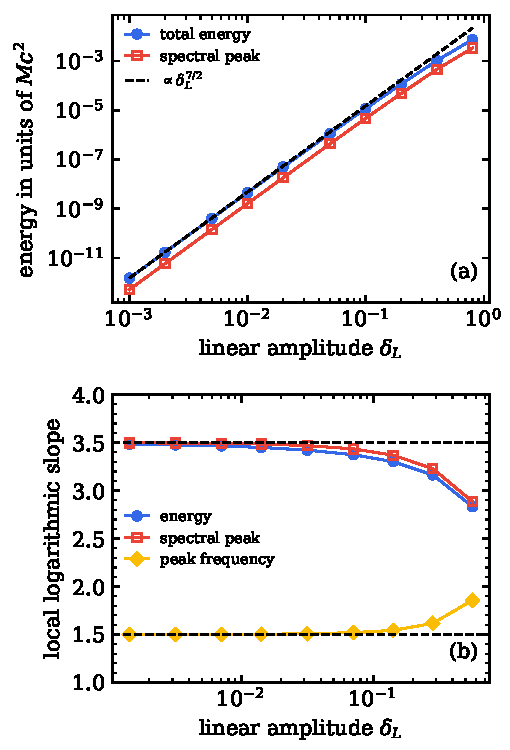
\includegraphics[width=\columnwidth]{fig_baseline.pdf}
\caption{Semi-analytic Newtonian baseline: a Zel'dovich ellipsoid with the quadrupole formula. (a) Radiated energy and spectral peak against the linear amplitude, with the $7/2$ power law. (b) Local logarithmic slopes of the energy, the peak and the peak frequency; dashed: $7/2$ and $3/2$.}
\label{fig:baseline}
\end{figure}

Two comparisons with the literature are open. The shell-crossing times of Ref.~\cite{Escriva:2026gw} are reproduced closely only by a literal reading of its force law, in which the patch also attracts the background inside it, and the prefactor of the peak energy density of Ref.~\cite{Dalianis:2024gw} is missed by a factor between one and four hundred, with the cause unknown. The Newtonian $N$-body baseline in the code's Newtonian mode replaces these readings at the next gate.

\subsection{Independent rechecks}\label{sec:recheck}

Every result above was recomputed by a second agent from a clean export of the committed scripts and reproduced to the last bit; the key derivations (the plane-symmetric null, the crossed-wave strain, the polarization sign, the Zel'dovich energy, the sheet modes and the closed-box backreaction) were redone with code written independently of the first agents. The figures of this note were drawn from the outputs of the registered runs, each checked against the checksum its run recorded where one exists and against the copy committed by the run's package.

\section{Plan and open questions}\label{sec:plan}

The rows of the program's verification suite held by this track are the matter-era background, the growth of linear perturbations, linear waves in a periodic box, the plane-symmetric pancake through shell crossing, the weak-field multi-code comparison, and, shared with the primordial-black-hole track, Szekeres-type dust. Under the program's ruling the multi-code row is the shearing-dust comparison of Ref.~\cite{Adamek:2020shearing}, run in this code against its published numbers, together with full relativity against the Newtonian mode of the code on the same particles. Figure~\ref{fig:timeline} places the gates in time.

\begin{figure*}[t]
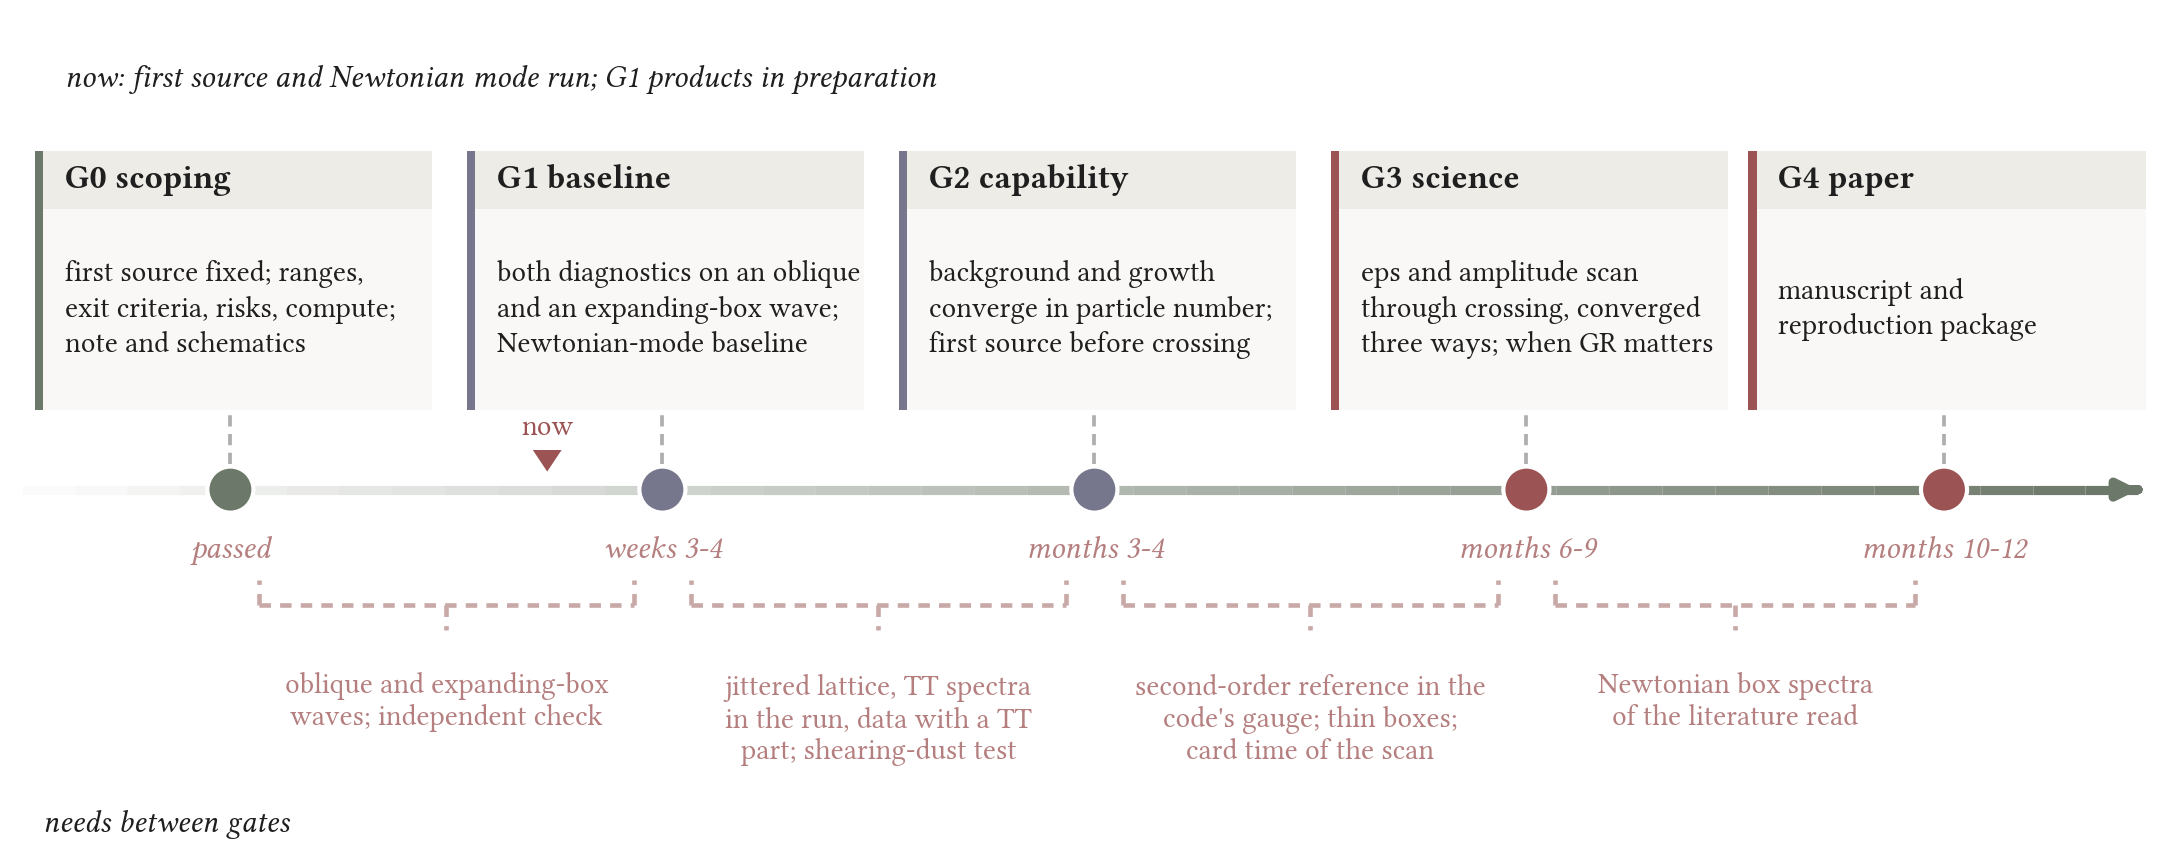
\includegraphics[width=\textwidth]{schem_timeline.png}
\caption{Stage timeline of the track. Circles: the five gates at their target times (green: scoping; slate: baseline and verified capability; red: science and paper). Boxes: what each gate requires. Dashed brackets: what the step between two gates needs.}
\label{fig:timeline}
\end{figure*}

The next runs are the first-source scan: the crossed waves with $\epsilon=0$, $0.1$, $0.3$ and $1$ at $\delta=0.01$ in the box of four initial Hubble radii, with two particles per cell and direction, dumps of the metric through shell crossing, and a second run of $\epsilon=1$ with a driven shift as the spatial-gauge leg. The predictions were written before the initial data were made: the null run carries no TT part at any nonzero wave number through crossing; before crossing the $(k,k,0)$ strain equals the crossed-wave strain times the junk solution, linear in $\epsilon$; the spatial-gauge piece of the flat projection, computed from the measured non-TT part, stays small before crossing and accounts for the difference between the two spatial gauges. The same correction applied to the earlier three-wave dumps decides whether their late rise is a gauge effect.

Open at this stage, in the order in which they block the gates: the oblique-wave test and a wave in an expanding box with both diagnostics, which need the polarization fix of the upstream generator; the Newtonian-mode baseline of the plane wave and of the ellipsoid; a jittered particle lattice for the noise floor after shell crossing, the main risk of the problem; the second-order reference strain carried to the code's slicing, and the York TT part on the curved slice; the relativistic reference of the plane pancake from the planar Szekeres class; particle-number convergence of the background and of the growth rate; thin periodic boxes for the convergence leg at the finest resolution; the reading of the two Newtonian box results \cite{Eggemeier:2022gw,Fernandez:2023gw} and of the report of a secular third-order term, against which the relativistic spectrum is to be compared.

\section{Summary}\label{sec:summary}

A plane-symmetric pancake radiates nothing, because its symmetry leaves no transverse-traceless part at any wave number; the first source is therefore two crossed waves, whose single-wave member is the null and whose strain before crossing is fixed in closed form by the product of the two potentials. The code propagates gravitational waves in a periodic box with the errors its stencils predict, and two independent diagnostics read them off its output. The first full-relativity pancake runs through shell crossing with every particle kept; its departure from Newtonian gravity is a converged property of the solution that grows with the square of the box size in Hubble radii, and its constraint violation is the sampling error of a stretched lattice, which a finer lattice removes. What remains before the signal itself is measured is gauge: which part of a second-order TT strain in the code's coordinates is radiation.

\begin{acknowledgments}
The calculations, the code and this note were produced by large-language-model agents under human direction, within the numerical-relativity particle-in-cell cosmology program.
\end{acknowledgments}

\appendix

\section{Parameters}\label{app:parameters}

Table~\ref{tab:parameters} lists the physical and simulation parameters of the scenarios of this note.

% generated by scripts/ledger.py; do not edit
\begin{table*}
\caption{Parameters of the scenarios.}
\label{tab:parameters}
\begin{ruledtabular}
\begin{tabular}{lll}
Scenario & Parameter & Value \\
\hline
Linear wave, vacuum box & box side $L$ & one wavelength \\
 & amplitude $A$ & $1\times10^{-6}$ \\
 & cells per wavelength $N$ & 16, 32, 64, 128 \\
 & duration & ten crossings (two for the dumps) \\
 & slicing; shift & conformal time; zero \\
Oblique flat wave & box; wave vector & unit box; $2\pi(1,1,1)$ \\
 & amplitudes $+$, $\times$; their relative phase & $10^{-6}$, $5\times10^{-7}$; 1 rad \\
 & cells per side; duration & 16, 32, 48, 64; four periods ($t=2.3094$) \\
 & slicing; shift & conformal time; zero \\
Expanding-box standing mode & box side (initial Hubble radii); wave vector & 4; $(\pi/2)(1,1,0)$ \\
 & initial $h'$ amplitudes $+$, $\times$; relative phase & $2\times10^{-6}$, $10^{-6}$; 1 rad \\
 & matter; cells per side & one particle per cell, at rest; 16, 32, 48, 64 \\
 & end & $t=10$, $a=36$ \\
Plane-wave pancake & amplitude $\delta$ at $a=1$ & 0.05 \\
 & box side (initial Hubble radii) & 1 and 4 \\
 & cells per side & 32, 64, 96 (box 1); 64 (box 4) \\
 & particles per cell & 1; 8 (two per direction, 64 cells) \\
 & end & $a=42$, twice the first crossing \\
 & slicing; shift & conformal time; zero \\
First source (crossed waves) & amplitude $\delta$; ratios & 0.01; $(1,\epsilon,0)$ \\
 & $\epsilon$ & 0, 0.1, 0.3, 1 \\
 & second amplitude $\delta$ ($64^3$, $\epsilon=1,0.3$) & 0.0025 \\
 & jittered nulls ($\epsilon=0$, $64^3$): jitter along $y$, $z$ & 0.3 and 0.1 cells \\
 & box side (initial Hubble radii) & 4 \\
 & cells per side; particles per cell & 64 and 32; 8 \\
 & end; dump interval in conformal time & $a=140$; 0.1 \\
 & slicing; shift & conformal time; zero (also driven, $\epsilon=1$) \\
Newtonian pancake & amplitude $\delta$ at $a=1$; box side & 0.05; one length unit \\
 & cells per side; particles per cell & 16, 32, 64; 1 \\
Newtonian ellipsoid & model & C of Ref.~\cite{Escriva:2026gw}, from turnaround \\
 & turnaround time; deformation $\alpha_{\rm e}$ & 9.53\,$t_k$; 0.111 \\
 & cells per side; particles per cell & 32, 64, 128; 8 \\
 & rescaled copies $\alpha_{\rm e}$ & 0.05, 0.1, 0.2 \\
\end{tabular}
\end{ruledtabular}
\end{table*}


\section{Numerical ledger}\label{app:ledger}

Table~\ref{tab:ledger} gives every number behind this note with the registered run that produced it. The outputs of each run are checked against the checksums the run recorded, where it recorded them, and against the copies committed by the run's package. The statements taken from papers were read at their sources: the $7/2$ scaling in Ref.~\cite{Dalianis:2024gw}, \texttt{pII\_GW\_Vir\_C2\_Arx.tex} line 1074; the crossing times and the peculiar speeds of Ref.~\cite{Escriva:2026gw}, \texttt{main\_v3.tex} lines 2276--2279 and 2395--2405, its redshift coefficient at line 2542; the energy density of the TT part, Ref.~\cite{Ota:2021tt}, \texttt{prd\_v1.tex} lines 258--262; the tensor equation, Ref.~\cite{Adamek:2016gevolution}, \texttt{compendium\_arxiv.tex} lines 142 and 294--298; the methods of the two box calculations, Refs.~\cite{Eggemeier:2022gw,Fernandez:2023gw}, from their abstracts, \texttt{main.tex} line 82 and lines 107--115. The fourth-order mesh convergence of the homogeneous background is the earlier mesh study of the cosmology extension (its analysis file \texttt{cosmo/analysis/daverio\_a.json}), re-read by the track. The figures and tables were made from these runs in the registered run of the note package named in its journal. Of the 28 numbers and statements of the track's stage documents of the first stage check that were checked against these files, 24 agree at the precision stated and 4 differ%
: the order of magnitude given for the lapse error of the homogeneous run at the smaller scale factor; the agreement with the Fourier-symbol prediction, stated without the larger departure of the phase error at the finest resolution; the Hamiltonian constraint of the earlier mesh study, quoted for a thousandfold expansion with the values of its first record, while at the end of that expansion it stops falling between the two finest meshes; and the Newtonian mode of the code, described as absent from the main branch, a statement written before the first wave of the program was merged. In each case the files hold, and the sentences of this note follow them.

% generated by scripts/ledger.py from registered run outputs; do not edit
\begin{table*}
\footnotesize
\caption{Numerical ledger. Every number behind this note with the registered run that produced it.}
\label{tab:ledger}
\begin{ruledtabular}
\begin{tabular}{p{0.47\textwidth}p{0.24\textwidth}l}
Quantity & Value & Run \\
\hline
\multicolumn{3}{l}{\emph{Linear wave in the periodic vacuum box (ten crossings)}} \\
amplitude error, cosmology numerics, $N=16,32,64$ & -0.000172, $-1.49\times10^{-6}$, $-1.48\times10^{-8}$ & \texttt{\scriptsize B-emd-gw-20261115-131016-03b1119} \\
phase error (rad), cosmology numerics, $N=16,32,64$ & -0.000249, $-6.25\times10^{-6}$, $-2.63\times10^{-7}$ & \texttt{\scriptsize B-emd-gw-20261115-131016-03b1119} \\
measured orders, amplitude 16--32, 32--64; phase 16--32, 32--64 & 6.85, 6.65, 5.32, 4.57 & \texttt{\scriptsize B-emd-gw-20261115-131016-03b1119} \\
amplitude error, upstream test numerics, $N=16,32,64$ & -0.00879, -0.000284, $-8.92\times10^{-6}$ & \texttt{\scriptsize B-emd-gw-20261115-131016-03b1119} \\
phase error (rad), upstream test numerics, $N=16,32,64$ & -0.00829, -0.000523, $-3.26\times10^{-5}$ & \texttt{\scriptsize B-emd-gw-20261115-131016-03b1119} \\
measured orders, upstream numerics, as above & 4.95, 4.99, 3.99, 4 & \texttt{\scriptsize B-emd-gw-20261115-131016-03b1119} \\
largest relative departure from the Fourier-symbol prediction, $N\le64$: amplitude, phase (cosmology); amplitude, phase (upstream) & 0.00854, 0.0955, 0.00231, 0.00602 & \texttt{\scriptsize B-emd-gw-20261115-131016-03b1119} \\
amplitude and phase error at $N=128$ (rounding floor of $1+h$) & $3.65\times10^{-9}$, $-8.59\times10^{-8}$ & \texttt{\scriptsize B-emd-gw-20261115-131016-03b1119} \\
$\int\mathcal H^2$ of the generator's oblique data, $k=(1,1,1)$; axis-aligned & $1.39\times10^{-9}$, $3.94\times10^{-22}$ & \texttt{\scriptsize B-emd-gw-20261115-131016-03b1119} \\
largest $|e_{ij}k^j|$ of the generator's tensor over random directions; with two signs flipped & 1, $3.76\times10^{-16}$ & \texttt{\scriptsize B-emd-gw-20261115-131027-03b1119} \\
gauge wave, $A=0.01$: orders of the metric error and of $\mathcal H$, $N=50\to100$ & 5.66, 5.92 & \texttt{\scriptsize B-emd-gw-20261115-131016-03b1119} \\
\multicolumn{3}{l}{\emph{Diagnostics}} \\
analytic random waves: number of modes; largest relative error of the shell energies & 48, $2.63\times10^{-12}$ & \texttt{\scriptsize B-emd-gw-20261115-131016-03b1119} \\
AthenaK wave at $t=2$, 32 cells: amplitude, phase (rad), energy density; largest $\Psi_4$ error over the dumps & $2.97\times10^{-7}$, $1.25\times10^{-6}$, $5.93\times10^{-7}$, $1.43\times10^{-6}$ & \texttt{\scriptsize B-emd-gw-20261115-120128-7dfaa38} \\
lag of the code's own Weyl output (steps); step size & -7, 0.00781 & \texttt{\scriptsize B-emd-gw-20261115-120128-7dfaa38} \\
earlier three-wave relativistic dumps (two deposits): rms $h^{\rm TT}$ at $a\approx36$; $a$ of the last dump; rms $h^{\rm TT}$ there; square of the rms non-TT part there & $1.21\times10^{-9}$, $1\times10^{3}$, $2.49\times10^{-9}$, $1.28\times10^{-9}$, $1.22\times10^{-9}$, $1\times10^{3}$, $4.31\times10^{-9}$, $1.34\times10^{-9}$ & \texttt{\scriptsize B-emd-gw-20261115-120846-d1509b5} \\
the same dumps at $a\approx1000$, two deposits: rms $h^{\rm TT}$; rms of the spatial-gauge piece; rms after its removal; kinetic over gradient energy of the TT part & $2.49\times10^{-9}$, $2.06\times10^{-10}$, $2.5\times10^{-9}$, 0.017, $4.31\times10^{-9}$, $2.23\times10^{-10}$, $4.32\times10^{-9}$, 0.0188 & \texttt{\scriptsize B-20261115-164616-a6d9477} \\
\multicolumn{3}{l}{\emph{First source and regime}} \\
largest relative departure of the $(k,k,0)$ amplitude from $\frac{5}{12}|\phi_x\phi_y|$; largest TT strain of the plane wave & $3.33\times10^{-16}$, 0 & \texttt{\scriptsize B-emd-gw-20261115-113148-4e5c33b} \\
Fourier amplitude at $(k,k,0)$, three-wave data, $\delta=0.01$, $L=4$ & $1.39\times10^{-5}$ & \texttt{\scriptsize B-emd-gw-20261115-113148-4e5c33b} \\
independent rederivation: real cosine amplitude of $h_+$; relative difference & $-2.77\times10^{-5}$, $1.22\times10^{-16}$ & \texttt{\scriptsize B-emd-gw-20261115-131027-03b1119} \\
symbolic: TT projection vanishes for $E(2)$-symmetric data; growth law forced on a flat transverse slice & \texttt{\scriptsize yes}, \texttt{\scriptsize $\dot D=-\tfrac32 D\,\dot a/a$} & \texttt{\scriptsize B-emd-gw-20261115-113102-bc5e082} \\
junk TT of conformally flat data: logarithmic slope of the envelope, $10<a<100$; envelope at $a=60$ over the static value & -0.997, 0.0182 & \texttt{\scriptsize B-emd-gw-20261115-113632-2960145} \\
$\omega_{\rm vir}/(ck_1)$ for $\delta=0.0025$--$0.05$, box of four Hubble radii & 0.81, 3.57 & \texttt{\scriptsize B-emd-gw-20261115-113632-2960145} \\
card-hours per run, $\delta=0.01$ to $a=140$: $64^3$, $128^3$, $256^3$, $256^2\times16$ & 0.0175, 0.362, 5.79, 0.362 & \texttt{\scriptsize B-emd-gw-20261115-113632-2960145} \\
the same, $\delta=0.0025$ to $a=560$ & 0.0366, 0.757, 12.1, 0.757 & \texttt{\scriptsize B-emd-gw-20261115-113632-2960145} \\
\end{tabular}
\end{ruledtabular}
\end{table*}
\begin{table*}
\footnotesize
\caption{Numerical ledger (continued).}
\label{tab:ledger2}
\begin{ruledtabular}
\begin{tabular}{p{0.47\textwidth}p{0.24\textwidth}l}
Quantity & Value & Run \\
\hline
\multicolumn{3}{l}{\emph{Plane-wave pancake through shell crossing}} \\
first crossing of the exact Zel'dovich sheets, 64 sheets (scale factor) & 21 & \texttt{\scriptsize B-emd-gw-20261115-123852-ea4475c} \\
first crossing, relativistic, one Hubble radius, 32, 64, 96 cells (coordinate label) & 21.8, 21.4, 21.3 & \texttt{\scriptsize B-emd-gw-20261115-123852-ea4475c} \\
first crossing, Newtonian particle mesh, 32, 64 cells & 21.5, 21.2 & \texttt{\scriptsize B-emd-gw-20261115-123852-ea4475c} \\
four Hubble radii, 64 cells: coordinate label; proper time of the crossing sheets; the same for one Hubble radius & 22.8, 22.3, 21.3 & \texttt{\scriptsize B-emd-gw-20261115-123852-ea4475c} \\
relativistic minus Newtonian position at $a=10$: one Hubble radius, 32 and 64 cells; relativistic minus Zel'dovich, 96 cells; four Hubble radii; ratio of the two box sizes & 0.00322, 0.0032, 0.0032, 0.0517, 16.1 & \texttt{\scriptsize B-emd-gw-20261115-123852-ea4475c} \\
relativistic minus Zel'dovich at $a=10$, 64 cells, one and two particles per cell and direction & 0.0032, 0.00321 & \texttt{\scriptsize B-emd-gw-20261115-123852-ea4475c} \\
Newtonian minus Zel'dovich at $a=10$: 64 cells; 32 cells; 32 cells with two per cell and direction & 0.00102, 0.00205, 0.000408 & \texttt{\scriptsize B-emd-gw-20261115-123852-ea4475c} \\
mean $|\mathcal H|$ relative, $a=10,15$: one per cell; two per cell and direction (64 cells) & 0.000158, 0.00129, $3.22\times10^{-5}$, $4.25\times10^{-5}$ & \texttt{\scriptsize B-emd-gw-20261115-123852-ea4475c} \\
mean $|\mathcal M|$ relative, $a=15$: one; two per cell and direction & 0.211, 0.00631 & \texttt{\scriptsize B-emd-gw-20261115-123852-ea4475c} \\
ratio one to two per cell and direction at $a=15$: $\mathcal H$, $\mathcal M$ & 30.3, 33.5 & \texttt{\scriptsize B-emd-gw-20261115-123852-ea4475c} \\
largest mean $|\mathcal H|$ after crossing, $a=22$--$42$: one; two per cell and direction & 0.00706, 0.00203 & \texttt{\scriptsize B-emd-gw-20261115-123852-ea4475c} \\
plane symmetry: largest spread of $x$ over a lattice plane ($L$); largest transverse velocity & $4.51\times10^{-14}$, $1.25\times10^{-12}$ & \texttt{\scriptsize B-emd-gw-20261115-123852-ea4475c} \\
card-hours of the relativistic runs: one per cell; two per cell; total & 0.284, 0.197, 0.481 & \texttt{\scriptsize B-emd-gw-20261115-115217-69ab1db} \\
\multicolumn{3}{l}{\emph{Homogeneous background}} \\
largest relative lapse error, $a=4$ and $a=36$ (step limited); $\mathcal H$ at $a=36$ & $1.91\times10^{-7}$, $7\times10^{-8}$, $6.05\times10^{-8}$ & \texttt{\scriptsize B-emd-gw-20261115-115414-7ffbde1} \\
\multicolumn{3}{l}{\emph{Semi-analytic Newtonian baseline}} \\
largest departure of the local slopes from $7/2$, $3/2$, $7/2$ for $\delta_L\le10^{-2}$: energy, peak frequency, peak & 0.0337, 0.00126, 0.00649 & \texttt{\scriptsize B-emd-gw-20261115-115752-840e994} \\
self-similarity: relative spread of the energy coefficient over the amplitude & $2.59\times10^{-13}$ & \texttt{\scriptsize B-emd-gw-20261115-115752-840e994} \\
literal model B: first crossings along $x$, $y$ ($t/t_k$); relative difference from Ref.~\cite{Escriva:2026gw} & 22.8, 29.1, 0.0105, 0.000946 & \texttt{\scriptsize B-emd-gw-20261115-115752-840e994} \\
coefficient of the turnaround-to-reheating time ratio (21.03 in Ref.~\cite{Escriva:2026gw}) & 21 & \texttt{\scriptsize B-emd-gw-20261115-115752-840e994} \\
ratio of our $\Omega_{\rm GW}$ to the prefactor of Ref.~\cite{Dalianis:2024gw} (range over four parameters) & 144, 392 & \texttt{\scriptsize B-emd-gw-20261115-115752-840e994} \\
independent quadrature of the ellipsoid energy against the closed form & $2.22\times10^{-16}$ & \texttt{\scriptsize B-emd-gw-20261115-131027-03b1119} \\
second-order lapse of a closed box with a TT wave, $t=10$, $A=10^{-6}$: conformal time; 1+log & $-1.64\times10^{-10}$, $-9.87\times10^{-10}$ & \texttt{\scriptsize B-emd-gw-20261115-131027-03b1119} \\
\end{tabular}
\end{ruledtabular}
\end{table*}
\begin{table*}
\footnotesize
\caption{Numerical ledger: the crossed waves in full relativity.}
\label{tab:ledger3}
\begin{ruledtabular}
\begin{tabular}{p{0.47\textwidth}p{0.24\textwidth}l}
Quantity & Value & Run \\
\hline
\multicolumn{3}{l}{\emph{Crossed waves in full relativity ($\delta=0.01$, box of four initial Hubble radii, $64^3$ unless stated)}} \\
initial data: largest Hamiltonian and momentum residuals of the four cases; particles per run & $3.97\times10^{-11}$, $2.47\times10^{-16}$, 2097152 & \texttt{\scriptsize B-20261115-161656-03d75e1} \\
static amplitude $s$ at $\epsilon=1$; Zel'dovich first crossing $1+1/\delta$ & $-3.08\times10^{-5}$, 101 & \texttt{\scriptsize B-20261115-174722-ba1048d} \\
largest $|c_+/(s\epsilon g)-1|$, $2\le a\le10$: $\epsilon=0.1,0.3,1$ & 0.00224, 0.00222, 0.00435 & \texttt{\scriptsize B-20261115-174722-ba1048d} \\
the same at $(k,-k,0)$ with the opposite sign & 0.00224, 0.00222, 0.00435 & \texttt{\scriptsize B-20261115-174722-ba1048d} \\
the same at $(k,k,0)$, $32^3$ & 0.00195, 0.0019, 0.00379 & \texttt{\scriptsize B-20261115-184650-2d155b6} \\
departure from second order at $a=20$: $\epsilon=0.1,0.3,1$ & 0.0115, 0.0125, 0.0231 & \texttt{\scriptsize B-20261115-174722-ba1048d} \\
the same at $a=40$ & 0.0576, 0.062, 0.115 & \texttt{\scriptsize B-20261115-174722-ba1048d} \\
the same at $a=60$ & 0.145, 0.156, 0.301 & \texttt{\scriptsize B-20261115-174722-ba1048d} \\
logarithmic slope of the departure between $a=10$ and $a=60$ & 2.32, 2.36, 2.35 & \texttt{\scriptsize B-20261115-174722-ba1048d} \\
departure over $1+\epsilon^2$, relative to that of $\epsilon=0.1$: $\epsilon=0.3,1$ at $a=20$; at $40$; at $60$ & 1.01, 1.02, 0.998, 1.01, 0.996, 1.05 & \texttt{\scriptsize B-20261115-174722-ba1048d} \\
linearity, $2\le a\le10$: largest relative difference of $c_+/\epsilon$, $0.3$ and $1$ against $0.1$ & 0.000497, 0.00213 & \texttt{\scriptsize B-20261115-174722-ba1048d} \\
the same at $a=20$ ($0.3$; $1$) and $a=60$ ($0.3$; $1$) & 0.000978, 0.0115, 0.0095, 0.136 & \texttt{\scriptsize B-20261115-174722-ba1048d} \\
largest $c_+/s$ at $\epsilon=1$ and its $a$; $c_+/(s\epsilon)$ at the end, $\epsilon=0.1,0.3$ & 2.55, 123, 2.06, 2.2 & \texttt{\scriptsize B-20261115-180834-c77a132} \\
null $\epsilon=0$, all dumps to $a=140$: largest TT amplitude of $h$ (single, double precision), of $\tilde A$ (double); largest $z$ dependence & $2.77\times10^{-16}$, $2.05\times10^{-16}$, $1.08\times10^{-16}$, $1.96\times10^{-14}$ & \texttt{\scriptsize B-20261115-174722-ba1048d} \\
$32^3$ against $64^3$: largest $|c_+$ ratio$-1|$, $5\le a\le40$: $\epsilon=0.1,0.3,1$, driven shift & 0.000861, 0.000319, 0.000232, 0.00022 & \texttt{\scriptsize B-20261115-184650-2d155b6} \\
the same, largest over the four cases for $40<a\le80$; at $a=100$ & 0.016, 0.0318 & \texttt{\scriptsize B-20261115-184650-2d155b6} \\
share of the four box modes in the mean square TT strain: $a=10$ ($\epsilon=0.1,1$), $a=20$ ($0.1,1$) & 0.963, 0.929, 0.843, 0.737 & \texttt{\scriptsize B-20261115-174722-ba1048d} \\
largest kinetic over gradient energy of the TT part for $a\ge12$: $\epsilon=0.1,1$ & 0.00857, 0.00821 & \texttt{\scriptsize B-20261115-180834-c77a132} \\
card-hours of the scan: three cases; two gauges; total & 0.252, 0.174, 0.426 & \texttt{\scriptsize B-20261115-164059-d802e82} \\
\end{tabular}
\end{ruledtabular}
\end{table*}
\begin{table*}
\footnotesize
\caption{Numerical ledger: the spatial gauge and the Newtonian mode.}
\label{tab:ledger4}
\begin{ruledtabular}
\begin{tabular}{p{0.47\textwidth}p{0.24\textwidth}l}
Quantity & Value & Run \\
\hline
\multicolumn{3}{l}{\emph{Spatial gauge of the projection ($\epsilon=1$, two gauges, $64^3$ unless stated)}} \\
exact pure-gauge data: slope of $\Lambda h$ and of $\Lambda h-G$ in the gauge amplitude; with a slicing change, $\Lambda h-G$ & 2, 3, 2 & \texttt{\scriptsize B-20261115-164221-6a6b779} \\
largest $|G_{\rm tot}/c_+|$ for $a\le20$, zero shift: $\epsilon=0.1,0.3,1$ & 0.0055, 0.00596, 0.0112 & \texttt{\scriptsize B-20261115-174722-ba1048d} \\
the same at $a=40$ & 0.0163, 0.0185, 0.0397 & \texttt{\scriptsize B-20261115-174722-ba1048d} \\
gauge difference of $c_+$ over $|s|$, as projected, $a=5,10,20,40,60$ & 0.00121, 0.0036, 0.0147, 0.0487, 0.115 & \texttt{\scriptsize B-20261115-180834-c77a132} \\
the same after $G_{\rm tot}$ in each gauge & $1.95\times10^{-5}$, $7.64\times10^{-5}$, 0.000305, 0.00296, 0.012 & \texttt{\scriptsize B-20261115-180834-c77a132} \\
median of corrected over projected difference where the latter exceeds $10^{-3}|s|$: $64^3$, $32^3$; share of such dumps & 0.084, 0.0928, 0.89 & \texttt{\scriptsize B-20261115-180834-c77a132} \\
the same median with the quadratic piece alone: $64^3$, $32^3$ & 5.24, 5.32 & \texttt{\scriptsize B-20261115-180834-c77a132} \\
departure from $sg$ at $a=10$: as projected, corrected; at $a=20$: as projected, corrected & 0.00444, 0.00687, 0.0231, 0.0345 & \texttt{\scriptsize B-20261115-180834-c77a132} \\
rms non-TT part, zero shift over driven shift, $a\ge10$: smallest, largest ratio & 16.2, 52.2 & \texttt{\scriptsize B-20261115-180834-c77a132} \\
median relative gauge difference for $a\le64$: magnetic Weyl part; flat TT strain & 0.00121, 0.0139 & \texttt{\scriptsize B-20261115-180834-c77a132} \\
first-order slicing of the earlier three-wave runs, $1<a\le121$: largest correlation of $\delta\ln\alpha$ with $\delta\ln\gamma^{1/6}$; rms of $\delta\ln(\alpha\gamma^{1/6})$ over that of $\delta\ln\alpha$, smallest and largest & -0.999, $5.48\times10^{-5}$, 0.0408 & \texttt{\scriptsize B-20261115-170610-c82b10c} \\
\multicolumn{3}{l}{\emph{Newtonian mode of the code}} \\
force excess $[(k\Delta x/2)/\sin(k\Delta x/2)]^2-1$ on the box mode, $N=16,32,64$ & 0.013, 0.00322, 0.000804 & \texttt{\scriptsize B-20261115-190015-4dd3416} \\
measured over predicted sheet error at $a=2,5$: $N=16$; $32$; $64$ & 0.9839, 0.9822, 0.9891, 1.019, 0.9999, 1.012 & \texttt{\scriptsize B-20261115-173904-a7297e3} \\
sheet error over displacement at $a=2$ ($N=32,64$), $a=5$ ($32,64$); ratios $32/64$ at $a=2,5$ & 0.00139, 0.000351, 0.00299, 0.000742, 3.96, 4.03 & \texttt{\scriptsize B-20261115-173904-a7297e3} \\
spectral particle mesh, the same: $a=2,5$ at $N=32$; at $N=64$ & 0.000109, 0.000606, $4.82\times10^{-5}$, 0.000327 & \texttt{\scriptsize B-20261115-173904-a7297e3} \\
measured over predicted at $a=10,15$, $N=32$ & 1.08, 1.2 & \texttt{\scriptsize B-20261115-173904-a7297e3} \\
first sheet crossing (scale factor): $N=16,32,64$; particle mesh $N=32,64$ & 21.87, 21.34, 21.16, 21.55, 21.22 & \texttt{\scriptsize B-20261115-173904-a7297e3} \\
largest spread of $x$ over a lattice plane ($L$) & $1.27\times10^{-15}$ & \texttt{\scriptsize B-20261115-173904-a7297e3} \\
rms relative error of the third derivative of $I_{xx}$, $1.2\le a\le15$: $N=16,32,64$ & 0.0926, 0.0235, 0.00613 & \texttt{\scriptsize B-20261115-173904-a7297e3} \\
Layzer--Irvine constant over largest $a|W|$: $N=16,32,64$ & $2.86\times10^{-6}$, $7.88\times10^{-7}$, $2.13\times10^{-7}$ & \texttt{\scriptsize B-20261115-173904-a7297e3} \\
ellipsoid: first crossing time ($t_k$), $N=32,64,128$; ODE; extrapolation and its order & 24.0659, 23.8955, 23.8604, 23.8524, 23.8513, 2.28 & \texttt{\scriptsize B-20261115-174405-af11300} \\
energy to the first crossing against the ODE, $N=32,64,128$; extrapolation; order & -0.344, -0.184, -0.0971, 0.0074, 0.876 & \texttt{\scriptsize B-20261115-174405-af11300} \\
ODE energy to the first crossing over $Mc^2$ & 0.000491 & \texttt{\scriptsize B-20261115-174405-af11300} \\
energy until one time unit before the crossing against the ODE (both averaged), $N=32,64,128$ & -0.102, -0.0151, -0.00265 & \texttt{\scriptsize B-20261115-174405-af11300} \\
relative change of the crossing time when the step is halved, $N=64$ & $2.07\times10^{-7}$ & \texttt{\scriptsize B-20261115-174405-af11300} \\
energy over $Mc^2(2\alpha_{\rm e})^{7/2}$, $N=32,64$; largest spread over four $\alpha_{\rm e}$; ODE value & 0.0618, 0.0764, $1.91\times10^{-14}$, 0.0946 & \texttt{\scriptsize B-20261115-174405-af11300} \\
card-hours of the $N=64$ pancakes & 0.0892 & \texttt{\scriptsize B-20261115-163653-f6324ea} \\
\multicolumn{3}{l}{\emph{Second readings of the wave-2 runs (own reader and reference)}} \\
largest departure from second order, $2\le a\le10$, $\epsilon=0.1,0.3,1$ & 0.00224, 0.00222, 0.00435 & \texttt{\scriptsize B-20261115-190007-e09a0d2} \\
ellipsoid first crossing time from the history files, $N=32,64,128$; extrapolation & 24.0659, 23.8955, 23.8604, 23.8513 & \texttt{\scriptsize B-20261115-190015-4dd3416} \\
largest relative spread of the self-similar energy over $\alpha_{\rm e}$ & $3.35\times10^{-14}$ & \texttt{\scriptsize B-20261115-190015-4dd3416} \\
\end{tabular}
\end{ruledtabular}
\end{table*}
\begin{table*}
\footnotesize
\caption{Numerical ledger: linear waves with both diagnostics.}
\label{tab:ledger5}
\begin{ruledtabular}
\begin{tabular}{p{0.47\textwidth}p{0.24\textwidth}l}
Quantity & Value & Run \\
\hline
\multicolumn{3}{l}{\emph{Linear waves with both diagnostics (oblique flat wave $F$, $N=16,32,48,64$ cells per side, last dump)}} \\
TT diagnostic, + polarization: amplitude error, $N=16,32,48,64$ & -0.000141, $-1.72\times10^{-6}$, $-1.57\times10^{-7}$, $-3.1\times10^{-8}$ & \texttt{\scriptsize B-20261119-164402-7438a99} \\
the same, phase error (rad) & 0.000253, $1.22\times10^{-5}$, $2.27\times10^{-6}$, $7.07\times10^{-7}$ & \texttt{\scriptsize B-20261119-164402-7438a99} \\
Fourier-symbol prediction written before the runs: amplitude, $N=16,32,64$; phase, $N=16,32,64$ & -0.000141, $-1.72\times10^{-6}$, $-3.17\times10^{-8}$, 0.000253, $1.22\times10^{-5}$, $7.03\times10^{-7}$ & \texttt{\scriptsize B-20261119-141844-2c5d622} \\
largest $|$measured over predicted$-1|$ over $N$: amplitude; phase & 0.0207, 0.00474 & \texttt{\scriptsize B-20261119-164402-7438a99} \\
local orders, amplitude (16--32, 32--48, 48--64); phase (the same) & 6.36, 5.89, 5.65, 4.38, 4.14, 4.06 & \texttt{\scriptsize B-20261119-164402-7438a99} \\
Weyl diagnostic (sixth-order stencils) minus TT, $N=16,32,48,64$ & $3.07\times10^{-5}$, $4.91\times10^{-7}$, $4.42\times10^{-8}$, $8.47\times10^{-9}$ & \texttt{\scriptsize B-20261119-164402-7438a99} \\
its local orders (16--32, 32--48, 48--64) & 5.97, 5.94, 5.74 & \texttt{\scriptsize B-20261119-164402-7438a99} \\
symbol error of the sixth-order first derivative at the wave, $N=16,32,64$ & $2.54\times10^{-5}$, $4.06\times10^{-7}$, $6.38\times10^{-9}$ & \texttt{\scriptsize B-20261119-141844-2c5d622} \\
largest difference of the Weyl and TT phase errors over $N$ (rad) & $1.6\times10^{-11}$ & \texttt{\scriptsize B-20261119-164402-7438a99} \\
Weyl diagnostic with spectral derivatives minus TT, largest over $N$ & $1.22\times10^{-11}$ & \texttt{\scriptsize B-20261119-164402-7438a99} \\
polarization ratio against the exact one, largest over $N$ and time: modulus; argument & $1.03\times10^{-9}$, $1.08\times10^{-9}$ & \texttt{\scriptsize B-20261119-164402-7438a99} \\
TT amplitudes at $t=0$ against the data, largest over $N$ (rounding) & $2.39\times10^{-11}$ & \texttt{\scriptsize B-20261119-164402-7438a99} \\
non-TT part over the wave at the end (second-order backreaction); TT content off the wave vector & 0.000144, $1.3\times10^{-9}$ & \texttt{\scriptsize B-20261119-164402-7438a99} \\
\multicolumn{3}{l}{\emph{Standing tensor mode of the expanding box ($X$, box of four initial Hubble radii, $t=10$, $a=36$)}} \\
TT diagnostic, $\times$ polarization: amplitude error, $N=16,32,48,64$ & $-7.05\times10^{-5}$, $1.32\times10^{-6}$, $4.25\times10^{-7}$, $1.4\times10^{-7}$ & \texttt{\scriptsize B-20261119-164402-7438a99} \\
the same, phase error (rad) & $8.3\times10^{-5}$, $3.06\times10^{-6}$, $5.88\times10^{-7}$, $2.76\times10^{-7}$ & \texttt{\scriptsize B-20261119-164402-7438a99} \\
prediction with the code's low-storage scheme on background and mode: amplitude, $N=16$--$64$; phase, the same & $-7.05\times10^{-5}$, $1.32\times10^{-6}$, $4.25\times10^{-7}$, $1.4\times10^{-7}$, $8.3\times10^{-5}$, $3.06\times10^{-6}$, $5.88\times10^{-7}$, $2.76\times10^{-7}$ & \texttt{\scriptsize B-20261119-153548-c7338f1} \\
largest $|$measured over predicted$-1|$: $\times$ amplitude, phase (all $N$); $+$ amplitude, phase ($N=16,32$) & $2.38\times10^{-5}$, 0.000115, 0.00528, 0.00796 & \texttt{\scriptsize B-20261119-164402-7438a99} \\
$+$ polarization, measured over predicted$-1$: amplitude at $N=48,64$; phase at $N=48,64$ & 0.0263, 0.0997, 0.102, 0.391 & \texttt{\scriptsize B-20261119-164402-7438a99} \\
measured over the first prediction (classical scheme, exact background)$-1$ at $N=32$: amplitude; phase & -0.204, -0.0446 & \texttt{\scriptsize B-20261119-164402-7438a99} \\
largest relative error of the scale factor, $N=16,32,48,64$ & $5.09\times10^{-8}$, $4.3\times10^{-8}$, $3.72\times10^{-8}$, $3.22\times10^{-8}$ & \texttt{\scriptsize B-20261119-164402-7438a99} \\
Weyl diagnostic (sixth order) minus TT, $N=16,32,48,64$ & $3.13\times10^{-5}$, $5.01\times10^{-7}$, $4.5\times10^{-8}$, $1.66\times10^{-8}$ & \texttt{\scriptsize B-20261119-164402-7438a99} \\
Weyl diagnostic with spectral derivatives minus TT: smallest, largest over $N$ & $1.91\times10^{-8}$, $2.41\times10^{-8}$ & \texttt{\scriptsize B-20261119-164402-7438a99} \\
argument error of the polarization ratio, largest over time, $N=16,32,48,64$ & $4.48\times10^{-9}$, $2.44\times10^{-8}$, $5.98\times10^{-8}$, $1.08\times10^{-7}$ & \texttt{\scriptsize B-20261119-164402-7438a99} \\
non-TT part over the mode envelope, largest; $\int\mathcal H^2$, largest & $3.11\times10^{-5}$, $9.01\times10^{-14}$ & \texttt{\scriptsize B-20261119-164402-7438a99} \\
card-hours of the two runs at $N=64$ & 0.0192 & \texttt{\scriptsize B-20261119-142124-feb2daf} \\
\end{tabular}
\end{ruledtabular}
\end{table*}
\begin{table*}
\footnotesize
\caption{Numerical ledger: the second round of the first source.}
\label{tab:ledger6}
\begin{ruledtabular}
\begin{tabular}{p{0.47\textwidth}p{0.24\textwidth}l}
Quantity & Value & Run \\
\hline
\multicolumn{3}{l}{\emph{Second round of the first source ($64^3$, eight particles per cell)}} \\
rerun of $\epsilon=1$ against the first run, largest relative difference of $c_+$ (double precision): $2\le a\le40$; $80\le a\le140$ & $9.5\times10^{-13}$, $4.71\times10^{-13}$ & \texttt{\scriptsize B-20261119-160607-ef83373} \\
two initial-data tools without jitter: largest difference of positions, velocities, masses and fields; particles & 0, 2097152 & \texttt{\scriptsize B-20261119-142727-02878d1} \\
jittered data: largest momentum residual, jitter 0.3, 0.1, none; largest Hamiltonian residual & 0.000763, 0.000283, $3.12\times10^{-17}$, $3.7\times10^{-11}$ & \texttt{\scriptsize B-20261119-141216-9c98929} \\
largest TT amplitude after the first dump: smallest and largest, jitter 0.3; the same, 0.1; quiet lattice, largest & $1.27\times10^{-7}$, $5.98\times10^{-7}$, $4.41\times10^{-8}$, $2.04\times10^{-7}$, $2.77\times10^{-16}$ & \begin{tabular}[t]{@{}l@{}}\texttt{\scriptsize B-20261119-160530-7bdcb45}\\\texttt{\scriptsize B-20261119-161519-6e0bc42}\\\texttt{\scriptsize B-20261115-174722-ba1048d}\end{tabular} \\
$|$measured$|/|$predicted$|$ at $(k,k,0)$, $3\le a\le20$: smallest, median, largest, jitter 0.3; the same, 0.1 & 0.927, 1.04, 1.33, 0.942, 1.03, 1.27 & \begin{tabular}[t]{@{}l@{}}\texttt{\scriptsize B-20261119-160530-7bdcb45}\\\texttt{\scriptsize B-20261119-161519-6e0bc42}\\\texttt{\scriptsize B-20261119-142733-932e595}\end{tabular} \\
the same at $(k,-k,0)$ & 0.741, 0.943, 1, 0.728, 0.951, 1.01 & \begin{tabular}[t]{@{}l@{}}\texttt{\scriptsize B-20261119-160530-7bdcb45}\\\texttt{\scriptsize B-20261119-161519-6e0bc42}\\\texttt{\scriptsize B-20261119-142733-932e595}\end{tabular} \\
largest $|$phase difference$|$ (rad): $(k,k,0)$ jitter 0.3, 0.1; $(k,-k,0)$ jitter 0.3, 0.1 & 0.364, 0.184, 0.0812, 0.0629 & \texttt{\scriptsize B-20261119-160530-7bdcb45} \\
box-mode amplitude, jitter 0.3 over 0.1, $1.5\le a\le20$: smallest, median, largest & 2.12, 2.56, 2.65 & \begin{tabular}[t]{@{}l@{}}\texttt{\scriptsize B-20261119-160530-7bdcb45}\\\texttt{\scriptsize B-20261119-161519-6e0bc42}\end{tabular} \\
jittered null (0.3) over the $\epsilon=0.1$ signal at $(k,k,0)$, largest for $a$ in 2--20, 20--80, 80--140 & 0.0148, 0.0251, 0.0314 & \begin{tabular}[t]{@{}l@{}}\texttt{\scriptsize B-20261119-160530-7bdcb45}\\\texttt{\scriptsize B-20261115-174722-ba1048d}\end{tabular} \\
rms TT of all modes over the second-order estimate, jitter 0.3, $3\le a\le20$: smallest, largest & 12, 14.7 & \begin{tabular}[t]{@{}l@{}}\texttt{\scriptsize B-20261119-160530-7bdcb45}\\\texttt{\scriptsize B-20261119-142733-932e595}\end{tabular} \\
share of the TT power at $|\mathbf k|L/2\pi\ge16$: jitter 0.3 at $a=2.3,12,140$; 0.1 at $a=2.3,12$; signal $\epsilon=0.1$ at $a=12,121$ & 0.984, 0.949, 0.61, 0.985, 0.952, $6.18\times10^{-12}$, $5.59\times10^{-5}$ & \texttt{\scriptsize B-20261119-161734-a3a1366} \\
kinetic over gradient energy of the TT part at $a=140$: jitter 0.3, 0.1 & 0.0115, 0.00925 & \begin{tabular}[t]{@{}l@{}}\texttt{\scriptsize B-20261119-160530-7bdcb45}\\\texttt{\scriptsize B-20261119-161519-6e0bc42}\end{tabular} \\
largest $a$ with departure $\le$ half a percent from $a=2$ on: $\delta=0.01$ ($\epsilon=1,0.3$); $\delta=0.0025$ ($\epsilon=1,0.3$) & 10.3, 12.6, 33.7, 41.7 & \begin{tabular}[t]{@{}l@{}}\texttt{\scriptsize B-20261115-180834-c77a132}\\\texttt{\scriptsize B-20261115-174722-ba1048d}\\\texttt{\scriptsize B-20261119-161519-6e0bc42}\\\texttt{\scriptsize B-20261119-163027-f0d304f}\end{tabular} \\
the same for one percent & 13, 17.7, 46.3, 63.3 & \begin{tabular}[t]{@{}l@{}}\texttt{\scriptsize B-20261115-180834-c77a132}\\\texttt{\scriptsize B-20261115-174722-ba1048d}\\\texttt{\scriptsize B-20261119-161519-6e0bc42}\\\texttt{\scriptsize B-20261119-163027-f0d304f}\end{tabular} \\
departure at $\delta=0.01$ over that at $0.0025$, $\epsilon=1$, $a=20,30,40,60$ & 17.9, 16.8, 17.2, 19.1 & \begin{tabular}[t]{@{}l@{}}\texttt{\scriptsize B-20261115-180834-c77a132}\\\texttt{\scriptsize B-20261119-161519-6e0bc42}\end{tabular} \\
the same, $\epsilon=0.3$ (at $a=20$ the smaller departure is at the rounding of the single-precision dumps) & 50.4, 16.8, 19.4, 18.3 & \begin{tabular}[t]{@{}l@{}}\texttt{\scriptsize B-20261115-174722-ba1048d}\\\texttt{\scriptsize B-20261119-163027-f0d304f}\end{tabular} \\
departure at $\delta=0.0025$ and $4a$ over that at $0.01$ and $a$, $a=10$--$35$: smallest, largest, $\epsilon=1$; the same, $0.3$ & 1.06, 1.47, 1.07, 1.31 & \begin{tabular}[t]{@{}l@{}}\texttt{\scriptsize B-20261115-180834-c77a132}\\\texttt{\scriptsize B-20261115-174722-ba1048d}\\\texttt{\scriptsize B-20261119-161519-6e0bc42}\\\texttt{\scriptsize B-20261119-163027-f0d304f}\end{tabular} \\
departure at $a=140$: $\delta=0.0025$ ($\epsilon=1,0.3$); $\delta=0.01$ ($\epsilon=1,0.3$) & 0.0939, 0.0505, 1.23, 1.15 & \begin{tabular}[t]{@{}l@{}}\texttt{\scriptsize B-20261119-161519-6e0bc42}\\\texttt{\scriptsize B-20261119-163027-f0d304f}\\\texttt{\scriptsize B-20261115-180834-c77a132}\\\texttt{\scriptsize B-20261115-174722-ba1048d}\end{tabular} \\
largest $|$departure$|$, $2\le a\le10$: $\delta=0.0025$ double precision ($\epsilon=1,0.3$); single ($1,0.3$); $\delta=0.01$ single ($1,0.3$) & 0.000317, 0.000349, 0.000956, 0.00266, 0.00435, 0.00222 & \begin{tabular}[t]{@{}l@{}}\texttt{\scriptsize B-20261119-161519-6e0bc42}\\\texttt{\scriptsize B-20261119-163027-f0d304f}\\\texttt{\scriptsize B-20261115-180834-c77a132}\\\texttt{\scriptsize B-20261115-174722-ba1048d}\end{tabular} \\
card-hours of the five runs of the round & 0.481 & \texttt{\scriptsize B-20261119-142833-19edd82} \\
second reading: numbers compared with the first-source package's own comparison files; largest relative difference & 30, $1.96\times10^{-12}$ & \begin{tabular}[t]{@{}l@{}}\texttt{\scriptsize B-20261119-163037-6553674}\\\texttt{\scriptsize B-20261119-164017-cd1ba52}\end{tabular} \\
\end{tabular}
\end{ruledtabular}
\end{table*}


\bibliography{references}

\end{document}
